\chapter{Scalable blockchain accounting}
\label{chap:implementation}

Trust and reputation systems rely heavily on interaction records. We have shown that the problem 
of recording transactions in distributed system has been in the focus of research for many years. 
The commercial interest has lately spawned many blockchain solutions. In previous work our 
research group has deployed a blockchain-based recording system for interactions, TrustChain. This system is 
implemented in a peer-to-peer video streaming service Tribler and the IPv8 project\footnote{https://github.com/tribler/py-ipv8}. 

This chapter introduces the blockchain and the TrustChain architecture itself to the reader. We argue
that the TrustChain is a more suitable system for a trust system than a single global ledger.
Also we analyze how the TrustChain architecture can be attacked. We point
out that although detection of attacks is possible the system does not incentivize agents to share 
and verify data which is essential for the detection. In the following chapter we analyze this in the
context of a model and propose an extension afterwards. 

% Although the exchange of information is part of those systems and as shown key to their manipulation
% resistance, exchanges are not explicitly recorded. 



% % 
% % Is this necessary??? 
% \section{Reciprocity}
% % 

% \subsection{Exchanges}
% As we have shown in Chapter \ref{chap:model}, the exchange of information is a major component of a trust 
% systems defense against manipulators and free-riders. Yet, TrustChain does not create records on 
% gossip. We identify this as a limitation. 

% Honest Tribler agents actually do exchange data in order to calculate a non-zero reputation for possible
% future peers. Still, without recording of this behavior, it cannot be rewarded or its absence be punished. 
% This is why we propose an extended TrustChain which enables recording of gossip and gossip-about-gossip. 
% The details of this extension are discussed in Section \ref{sec:extension}.

\section{Blockchain basics}
The design of distributed databases bears many challenges. Especially if sensitive data is involved
and users need to have access globally, the asynchrony of events, lack of guarantees on data 
consistency and agent honesty create issues. For the early years of the internet those challenges seemed
insurmountable. That is why most services that act on sensitive data are centralized, examples being 
banks, government institutions or commercial services like Facebook\footnote{https://facebook.com}.
Centralization has its own shortcomings such as abuse of power, dishonesty, single point-of-failure
and platform lock-in. We described those issues in more detail in Chapter \ref{chap:introduction}.
The increasing significance of those issues led to the design and implementation of the Bitcoin 
protocol~\cite{nakamoto2008bitcoin} for digital money transfers. The Bitcoin protocol allows a distributed network of agents 
to agree on the exact order of events, through a hash chain which acts as a distributed timestamp 
server and the proof-of-work algorithm. This architecture is commonly referred to as blockchain or
distributed ledgers.

\subsection{Concept}
A blockchain is essentially an append-only database in the form of chained blocks. It is designed to be
used as a secure information storage in distributed systems without any central governance. 

Each block on the chain contains a set of transactions, the root hash of that set, a nonce (used in 
the consensus algorithm) and the hash of the previous block. By including a hash from the previous block,
blocks are chained together as can be seen in Figure~\ref{fig:basic_blockchain}. Any 
change to a block on the chain will change the hash of that block. This voids the following block's
hash pointer because it points to the old block. 

The first block in the chain 
is called the genesis block. The Bitcoin blockchain and similar single-chain ledgers only have 
one genesis block. Each block can also be identified by a sequence number $s \in \mathbb{Z^\geq}$, which is an increasing 
integer that starts from 0 at the genesis block.

\begin{figure}
    \centering
    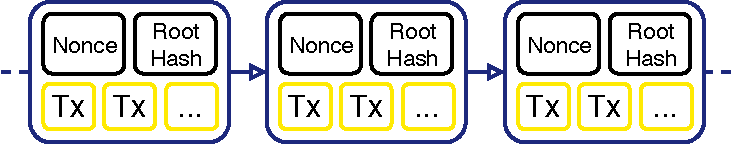
\includegraphics[width=0.7\textwidth]{images/blockchain.pdf}
    \caption{Conceptual depiction of a slice of a Bitcoin-like blockchain. Blocks contain multiple transactions and are chained together through the hash of the previous block. Source: \textit{Creation of TU Delft BLockchain Lab}}
    \label{fig:basic_blockchain}
\end{figure}

All agents are acting on the same copy of the blockchain. The one global chain therefore contains 
all transactions that happen on the network. Single global ledgers create an incentive for agents to publish new blocks by rewarding 
them with currency. New blocks are accepted if they are on top of the longest chain. This creates 
an incentive for all participating miners to stay up to date on the state of the global ledger. The
only way to create the next block and receive the block reward is acquire the latest state of the ledger.

% In order to allow for enough time to synchronize transactions and blocks, the difficulty of the puzzle 
% can be increased. This ensures a approximately fixed time between new blocks. This block time is 
% 10 minutes for Bitcoin. Together with the fixed block size the global transaction throughput of the
% system is capped. Research has shown that any proof-of-work system will not increase beyond a throughput
% of 60 transactions per second \cite{gervais2016security}. The scalability of the proof-of-work 
% algorithm is very limited which makes the Bitcoin solution only applicable in a context where high
% throughput 


\subsection{Consensus}
% why?: 
Transactions and new blocks need to be published  on the network. The block creation process
is managed by the consensus mechanism \textit{proof-of-work}. This process is also called mining and the nodes
that take part in it are thus miners. It works as follows: Each new block contains a computational 
intensive puzzle which needs to be solved in order to be able to publish a block. Specifically, 
miners are increasing the nonce $x$ until $\mathcal{H}(x) < d$ where $\mathcal{H}$ is any secure hash
function and $d$ is a target hash. The smaller $d$, the more hashes need to be calculated before finding a hash.
All miners are computing hashes until they find a correct $x$. 

Once they find a possible solution, the agent combines all the transactions that were published since the last
block and combines them to a new block. The block size is fixed such that after adding a certain number of 
transactions, the block is considered complete. If complete, the agent broadcasts the
block in the network. Any agent that receives the block will verify that
the solution to the puzzle is correct and all transactions are valid. If so, they add the new block
to their copy of the chain and start with solving the next puzzle in order to become the next 
creator of a block. 

The creator of the block is rewarded with transaction fees paid by the authors
of the included transactions and a coinbase transaction. The latter is the generation of new 
coins from a finite supply of new coins. Over time, the size of the coinbase transaction reduces 
until it reaches 0. At that point, miners are only rewarded with the transaction fees.

Conflicts can arise when two blocks are found at approximately the same time. Each block will be 
considered the latest by part of the network. The network is thus partitioned and a natural
fork is created in the chain. The conflict is resolved when the following blocks are mined. 
The partition with the larger CPU power will mine consecutive blocks faster. The longer
chain will persist as the other partition switches towards it. The mechanism ensures that (except for
the latest blocks) agents are acting on the same view of the network.

\subsection{Tamper-resistance}
% why?: show that the hash chain creates a tamper-proof record
The chain of hashes that connects blocks on the blockchain creates a theoretically tamper-proof history.  
Changes to any block will alter its hash and break the chain of hashes. Therefore any change to the 
block requires the recalculation of all following blocks. Because all blocks need to be agreed upon on the network 
other agents will be able to see such tampering with the blocks and will not agree on it. 

Similarly the order of blocks is ensured through the hash pointers. Any change to the order of blocks
will will result in a break in the hash chain.
The sequence of blocks also orders the transactions stored in the blocks. 
Any transactions in an earlier block happen before the transactions in the later block. Also, as was just 
explained, any change to the ordering of transactions. Even though this order
does not necessarily correspond to the local time of the agent who published the transaction, the 
blockchain will create a globally accepted order for transactions.  This is a major 
achievement because this order is robust against network delays, tampering and other attacks.

However, proof-of-work blockchain are not truly tamper-proof. The tamper-resistance is ensured through
mining power. As long as more than 50\% of the network's CPU power is controlled by honest agents, 
the correctness of the system is ensured. However, if any attacker is able to obtain a majority of
computing power, any tampering can be possible because the attacker can mine invalid blocks faster
then the honest minority. For very large networks such as the Bitcoin network, the probability of 
a single attacker having a majority of CPU power is very small. However, smaller networks or collusion
attacks in which multiple miners work together can be successful as shown by some examples~\cite{51percentbitcoingold, 51percentverge}.

The majority of the mining power can also be used to create a intentional fork in the chain in order 
to fix software bugs. If a majority of miners update their software to version that creates and verifies blocks
differently while a minority continues with the old software, a hard fork is created such that two
version of the blockchain are continued. Examples of this are Bitcoin Gold \footnote{https://bitcoingold.org} and Ethereum Classic \footnote{https://ethereumclassic.org}.

\subsection{Scalability}
A single global ledger like Bitcoin seems like a valid implementation for recording transactions for a
trust system. All transactions are exchanged with all agents on the network. The blockchain 
creates a totally ordered set of all global transactions which intrinsically means that each agent's 
transactions are also fully ordered. Double spend and forks are detectable through global consensus. 

However, the proof-of-work mechanism leads to issues in scalability. It restricts the global throughput
to at best 60 transactions per second~\cite{gervais2016security}. This is not enough to power a global-scale distributed trust 
system as we envision it. The proof-of-work consensus algorithm also leads a to a large expenditure of energy which creates 
large transaction costs. This is not acceptable if the trust system should be for general purpose 
applications. For example, users will not accept to pay for each video they stream on the Tribler 
platform. A different solution is therefore needed.

In Section \ref{sec:related_work} several improvements to the scalability are mentioned. Examples are
alternative consensus protocol such as proof-of-stake and delegated proof-of-stake. Also, sharding
and off-chain transaction channels have been proposed which are supposed to increase throughput.
Each solution balances three design variables: decentralization, scalability and consistency. This
is commonly called the scalability trilemma in blockchain communities \footnote{For example mentioned in the Ethereum wiki. https://github.com/ethereum/wiki/wiki/Sharding-FAQs}.
Crytpocurrencies generally target decentralization and consistency as the driving design factors. 
Financial transactions have high value and require consistency. Secure payments are enabled while 
scalability is less important.


\section{TrustChain}
\label{sec:trustchain}


TrustChain's design focus is in stark contrast with that of
Bitcoin. Instead of employing global consensus to guarantee a single global ledger, 
all agents in the TrustChain fabric are owner of a chain for themselves. This creates a scalable 
solution in which the total network throughput grows with the size of the network. However, the
scalability comes at the cost of consistency guarantees. 

We argue that when designing a global-scale
trust system, interaction throughput has higher value than consistency. Although undesired, we 
consider the manipulation of an agents reputation as less severe than stealing large amounts of 
money. Therefore, an architecture such as TrustChain with unbounded scalability is a better basis
for a trust system than single global ledgers.

We continue this chapter with a description of the TrustChain architecture.

\begin{figure}
    \centering
    \begin{subfigure}{0.49\textwidth}
        \centering
        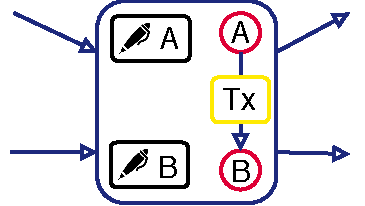
\includegraphics[width=0.8\textwidth]{images/block-2.pdf}
        \caption{Conceptual representation}
    \end{subfigure}
    \begin{subfigure}{0.49\textwidth}
        \centering
        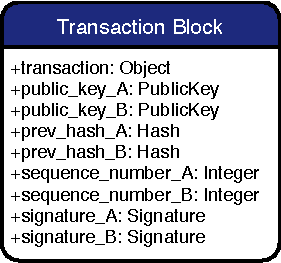
\includegraphics[width=0.6\textwidth]{images/transaction_block_data.pdf}
        \caption{Transaction block, data representation}
    \end{subfigure}
    \caption{A single block in the TrustChain fabric. Incoming arrows represent block hashes from the previous blocks of the agents' chains. Source: \textit{Creation of TU Delft BLockchain Lab}}
    \label{fig:trustchain_block}
\end{figure}

\subsection{Data structure}
\label{sec:transaction_blocks}
Similar to the Blockchain architecture TrustChain records transactions in blocks and links blocks 
with the use of hash pointers. Though, in contrast to having a single chain of blocks for the whole
network, in TrustChain each agent starts with an own genesis block. Hence, all agents record their
own transactions on their chain. 

Blocks in TrustChain contain exactly one transaction between two parties. Because both parties have 
their own chain and the transaction concerns both parties, any new block is added to both agents'
chains. Each block contains the following main elements:

\begin{itemize}
    \item \textbf{Transaction.} The transaction field records the value that was exchanged between agents.
    TrustChain is designed to be application agnostic. Thus the content of a transaction can be any 
    serializable data. 
    \item \textbf{Previous block hashes.} The hashes of the previous blocks of both agents' chains 
    firmly attaches the new block to their history. This is similar to the basic blockchain concept.
    \item \textbf{Public keys.} In order to uniquely identify the two agents that conduct a transaction
    their public keys are recorded.
    \item \textbf{Signatures.} Both agents provide a digital signature of the transaction with their 
    private key which any agent can check with the agents' public keys. This authenticates the 
    transaction and cryptographically proves that the real owners of the private key conducted the 
    transactions.
    \item \textbf{Sequence numbers.} All blocks on an agent's chain have a unique sequence number 
    which shows the position in the chain. 
\end{itemize}

A simplified depiction and data representation of a TrustChain block is shown in Figure~\ref{fig:trustchain_block}. When 
looking at a single agent the given data structure creates a chain of blocks which describes all the
transactions of that agent. However the second incoming and outgoing edge of each block entangles an
agent's chain with those of all partners. When looking at a complete network, of the transactions the
represents a directed acyclic graph(DAG). Such a structure is shown in Figure~\ref{fig:trustchain_graph}.

\begin{figure}
    \centering
    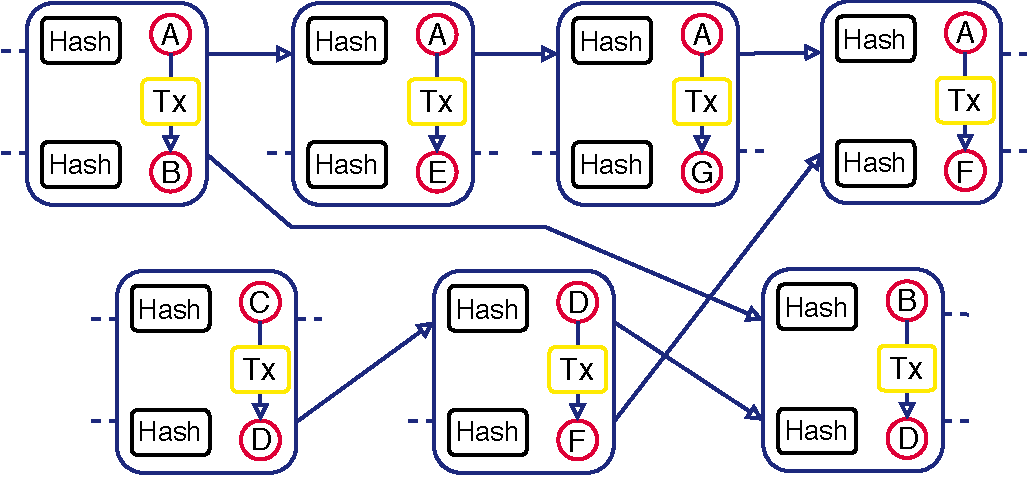
\includegraphics[width=\textwidth]{images/trustchain_graph.pdf}
    \caption{TrustChain graph structure with multiple transactions. The top row shows the chain of
    an agent A with links to multiple other blocks. Source: \textit{Creation of TU Delft BLockchain Lab}}
    \label{fig:trustchain_graph}
\end{figure}


\subsection{Verification protocol}
\label{sec:validation}
TrustChain blocks are designed in a way to be verified by any other node. The verification is 
required to ensure that the block has not been tampered with and is correctly connected to a valid 
chain. A block can only be valid if all of the following conditions are true:

\begin{enumerate}
    \item The transaction field contains the necessary information to properly define a transaction 
    in the application context. For Tribler it needs to contain at least the amount of data which 
    was uploaded and downloaded between the two agents. 
    \item Both block hashes need to point to the valid, previous block on the chain of the same 
    public key. This makes the validity a recursive definition which depends on the previous content
    of the chain of both agents.
    \item Both public keys need to be valid public keys.
    \item The signatures need to be correct for the given public keys and block content.
    \item The block needs to carry the next integer as sequence number compared to the blocks that 
    the previous hashes point to.
\end{enumerate}

The true validity of a block can only be established if the verifier also checks all other blocks on
the chains of both parties. Yet, that implies to check all other blocks of their partners and their
partners. Such a strong form of validity can thus only be ensured by verifying an exponentially 
growing amount of blocks.
% A block can only be valid if the hash pointers also point at valid blocks. This recursive definition
% requires agents to either verify the complete chain of both agents up to the block to be verified or
% assume that all previous partners have also verified their transactions. 

A weaker form of validity can be that the previous blocks pointed at, exist. That does not ensure 
the validity of the complete chain but allows for a simple non-recursive validity check.

\subsection{Tamper-evidence}
\label{sec:tamper-proof}
Blocks of the TrustChain architecture are tamper-evident. Blocks are chained through hashes of their
content and signed by both transaction parties. Any change to the content of the block, that is the
transaction field, the sequence numbers, the signatures, previous hashes or public keys will change
the hash of the block. Also, any such change will invalidate the original signatures of both agents. An agent
can renew her own signature but not the signature of the partner without access to the 
partner's private key. Apart from the invalid signatures also any consecutive block's previous hash
will be invalid because the tampered block's hash has changed.

We can conclude that any tampering of a block will be evident to an agent that performs verification
of the signatures and hash pointers of consecutive blocks.

\subsection{Scalability}
\label{sec:trustchain_scalability}
For a transaction to be successful in TrustChain, only the involved agents need to agree on the content. This
means that only two agents need to communicate to confirm a transaction. Transactions do not need to 
be publicly announced or sent to all nodes on
the network. Also, multiple transactions can be performed at the same time globally without breaking
the rules of the system. In contrast to the Bitcoin system, only the transactions of each agent are
strictly ordered, the global set of transactions is not.

This results in a system that scales with the size of the network. A simple example makes this very 
clear. Consider two networks, one with 10 nodes and one with 100 nodes. For simplicity we consider
time to be discrete and agents to interact in rounds. Each transaction takes 1 round and all agents 
interact. Throughput calculation is then straightforward. Nodes arrange in pairs and perform a
transaction. The small network will have 5 pairs and thus 5 transactions per round, while the large
network has 50 pairs and transactions. Although this example is extremely simplified, no real-world
effect like network delays, network churn or bandwidth restrictions greatly conflict with this property.

TrustChain does not include a global consensus and thus does not expend bandwidth, storage and 
computational power to create a global order for transactions. That removes the most costly component
from the general blockchain architecture. Without the expense of CPU power to calculate hashes as in the proof-of-work mechanism,
transactions only cost the bandwidth and computational expense of communicating with 
the direct interaction partners. TrustChain enables free transactions in a global distributed 
system with scaling throughput based on the network size. Hence, TrustChain is valid solution for a
global trust system.

\subsection{Security}
The superior scalability of the TrustChain architecture compared to single global ledgers comes at 
the expense of some security guarantees.

Similar to a single Blockchain the graph structure of TrustChain creates a tamper-proof record of
transactions. A large difference is that each agent reigns over a chain. Each agent seemingly is 
able to reorder transactions but blocks are signed by a second agent and the signature will become
invalid if the blocks are tampered with. Also blocks contain the previous hash of the counter party's
previous block. That ensures that the hashes cannot change without the other agent being able to 
detect the tampering.Therefore transactions are still recorded in a tamper-proof data structure.

Still, detectabillity does not ensure detection. The can only be secured if agents
continuously verify their partners data. Also, as the validity of a block is recursively defined, 
agents can only ensure the validity of a partners previous transaction if they possess their complete
chain and verified that chain. It is even harder to defend against attacks in which agent do not 
directly manipulate the data structure but make use of the incomplete knowledge which is intrinsic 
to distributed networks. 

% A prominent example, the double spend attack, has been defined and extensively 
% discussed in Chapter~\ref{chap:model}. We have shown that gossiping, that is sharing of knowledge, 
% is a way to detect such attacks. The current
% TrustChain system does not record gossiping in any way. Therefore agents do not have a strong 
% incentive to perform gossiping. In the next section an extension will be discussed which adds the 
% possibility of recording exchanges.

\section{Security analysis}
\label{sec:attacks}
If the trust system works as expected, a good reputation should have value to agents. All agents on 
the network attempt to obtain a good reputation and be seen as a trusted partner. As such their 
behavior should be meticulously agree with the rules. Yet, if the value is large enough and behaving
well comes at a large enough cost, agents will aim to bend the rules or even break them in a smart 
way in order to get the good reputation for free. As a designer of the trust system it is essential
to predict the possible ways of manipulation and prevent them. In this section we will define several
known types of attacks on trust systems and if applicable define how TrustChain can prevent them.

\subsection{Block manipulation}
\label{sec:tampering}
Block manipulation has been introduced previously. An agent changes a property of a block in his 
chain, distorting the true history in order to gain an advantage. For example, a block records a 
transaction in Tribler in which agent $A$ downloaded from agent $B$. The transaction reduces the 
reputation of agent $A$ which is why $A$ could decide to change the amount of data downloaded to 0.
If agent $A$ does this before the signatures are provided, $B$ will not agree to sign the transaction
and will ignore $A$ in the future because $A$ obviously is not an honest partner. On the other hand,
if both agents sign the transaction first, $A$ can change the value on his own chain without $B$ 
immediately noticing. The signature of $B$ however becomes invalid because $B$ signed the original, 
correct version of the block. In any following transaction, any agent $C$ that is about to interact
with $A$ has the chance to detect this fraud by checking the signatures on all previous transactions
of $A$. 

TrustChain makes any manipulation detectable. Still if agent $C$ collaborates with agent $A$ or 
agent $C$ is ``lazy'' and does not obtain $A$'s chain to verify it prior to an interaction, $C$ can 
perform a transaction. The collusion or laziness cannot be detected and $C$ will remain honest 
in the eyes of future partners.

\subsection{Forking and double-spending}
Forking is one of the most well-known attacks of blockchain based systems. In the cryptocurrency 
context it is also known as double spending. An attacking agent 
performs two conflicting transactions with two different partners. This translates to two transaction
blocks which have the same sequence number for an attacking agent $A$. Partner $B$ and $C$ are each
not aware of the other version of the block and will sign the block. This allows to ``overwrite''
a negative transaction (with $B$) with a positive transaction (with $C$). $A$ will only keep the positive transaction on 
the chain. 

TrustChain makes this attack detectable through the sequence number of the blocks. If any agent 
obtains both versions of the block, that agent will see that $A$ has signed and thus authorized the
creation of two blocks with the same sequence number. Also if $B$ obtains any later blocks from $A$ 
the hashes will not point to the transaction with $B$.  This creates a \textit{proof-of-fraud}. 

The actual
detection of this attack requires agents to obtain transactions from their peers and compare those 
to existing blocks. Because no agent is aware of the transaction with $B$, agents cannot not specifically 
request $B$'s history to check for the attack. Therefore, the detection requires the collaboration
of the network in the form of random block requests. As we will show in Chapter \ref{chap:model}, 
without exchanging information about their transactions, agents are not able to find a double-spender.

\subsection{Block withholding}
Once agents have a longer history they will have records of positive and negative encounters. A 
malicious agent then might try to hide any records of negative encounters, thus boosting the trust 
others have in the attacker. The architecture of TrustChain makes such an attack easily detectable.
The blockchain of any agent creates a tamper-proof, irreversible order for all transactions. Only if
the sequence numbers increase exactly by one to each following block can another agent be sure that 
the whole history was shared by an agent. Therefore to establish the trustworthiness of an agent, 
another agent at least needs to obtain their full chain.

Note that if an agent witholds the latest blocks, this cannot be detected by another agent (except
if that information was obtained already through gossiping). Yet such an attack is similar to a
double-spend because any newly created block will conflict with those blocks that were withheld.

\subsection{Whitewashing}
Agents that have a significantly bad reputation such that finding interaction partners becomes difficult may decide to create a new 
identity for themselves. Thus, they can rid themselves from the bad reputation and start fresh. This 
type of attack is called whitewashing. In the currently deployed version of TrustChain in Tribler 
this attack cannot be prevented as the software is free and new agents do not need registering with
any central institutions.

Still the impact of such attacks can be limited by having some mistrust of new agents joining the 
network. In that case new agents need to ``pay their dues'' before being accepted by the network 
as equals. For example, assume honest agents only upload data to agents that are above a certain level
of reputation. Once an agent is below that boundary he needs to upload data before downloading again.
Also, new agents start at that boundary level of reputation. In that case whitewashing will not be
possible. However the question then remains how the system can be bootstrapped and maintained
active because with each new agent the overall network reputation decreases such that at some point
only uploading is possible but no agent is able to download.

\subsection{Sybil attack}
One of the most serious attacks on trust systems is the Sybil attack. In a Sybil attack, the attacker
creates a set of new fake agents, called the Sybils. Together with the attacking agent the set of 
agents is called a Sybil region in the network. The Sybils create transaction blocks  
between each other without actually performing the transactions with the goal of boosting the 
reputation of one of the agents in the Sybil region. The attack is successful as honest agents 
cannot distinguish between fake and real transaction records. Each Sybil has a valid public and private
key and is able to sign transaction blocks. They create valid transaction data without any neccessary
manipulation or proof-of-fraud.

Multiple ways have been explored to prevent this attack. One way is to analyze the network topology
and use it to detect Sybil regions. A trust mechanism such as NetFlow, which has been proposed in 
\cite{OTTE2017} is resistant against weakly beneficial Sybil attacks. Another way is to increase the cost of 
registering new identities in the system. If each registered public key needs to be anchored on a 
costly blockchain like Bitcoin, it becomes much harder to create a Sybil region. We leave this problem
to future research.

\subsection{Collusion}
\label{sec:collusion}
Attacks are called a collusion attack if multiple attackers work together to achieve a beneficial
situation for at least one of the colluders. Attacks such as those described above, 
can become more successful when multiple attacks collude. An example of this was given for block 
manipulation. If one agent manipulates a block and afterwards interacts with a colluder to share the
wrongly obtained positive reputation, the colluders chain seems completely valid to honest agents.

In TrustChain it is hard to detect such collusion because we do not know whether agents actually 
did not know about an attacker or just claim so. We will next look at an extended system which 
records the knowledge of agents. Although this creates protection against some collusion attacks, 
still not every collusion can be protected against.

\section{Chapter conclusion}
TrustChain is a scalable solution for tamper-evident recording of transactions in a distributed 
network. It therefore fulfills many of the requirements that we set for our system in the previous
chapter. However, TrustChain cannot in itself provide consistency of interactions as we have shown
with the discussion of the double-spend attack. We show in the next chapter that gossiping is a
valid solution to solve this problem. Still TrustChain provides no strong incentive for agents to 
gather blocks from their peers. This opens the system to free-riders who do not exchange information and verify 
blocks but remain honest in the eyes of their peers. 

Additionally, the lack of incentive for gossiping decreases the probability of indirect reciprocity
because agents are not aware of each others good or bad reputation.
As we have discussed in the previous chapter, global-scale trust system will mostly rely of indirect
reciprocity. Therefore the dissemination of data is essential to our system.

On the other hand, such a strong exchange policy leads to a challenging storage and bandwidth 
requirement. Each agent's subjective network state will approximate the complete networks data.